\section{Data Overview}\label{sec:data_overview}
For calibrating the ChemCam instrument, the ChemCam team has collected a large amount of data from a variety of samples on Earth\cite{wiensPreFlight3}.
This data is stored in a directory structure as shown in Figure~\ref{fig:directory_structure}.
For each sample, the data is split into five datasets, one for each location on the sample that was shot at by the laser.
Each dataset contains CCS data stored in a \texttt{.csv} file.

\begin{figure}[ht]
    \scalebox{0.8}{
    \begin{forest}
        for tree={
            font=\ttfamily,
            grow'=0,
            child anchor=west,
            parent anchor=south,
            anchor=west,
            calign=first,
            inner xsep=7pt,
            edge path={
                \noexpand\path [draw, \forestoption{edge}]
                (!u.south west) +(7.5pt,0) |- (.child anchor) pic {folder} \forestoption{edge label};
            },
            % style for your file node
            file/.style={edge path={\noexpand\path [draw, \forestoption{edge}]
                (!u.south west) +(7.5pt,0) |- (.child anchor) \forestoption{edge label};},
                inner xsep=2pt,font=\small\ttfamily
                            },
            before typesetting nodes={
                if n=1
                {insert before={[,phantom]}}
                {}
            },
            fit=band,
            before computing xy={l=15pt},
            }
        [samples
            [0.1tio2
                [2015\_03\_27\_132008\_ccs.csv, file]
                [2015\_03\_27\_132210\_ccs.csv, file]
                [2015\_03\_27\_132331\_ccs.csv, file]
                [2015\_03\_27\_132453\_ccs.csv, file]
                [2015\_03\_27\_132624\_ccs.csv, file]
            ]
            [cadillac]
            [$\vdots$, file]
            [wc3]
        ]
    \end{forest}
    }
\caption{Directory structure of the data.}
\label{fig:directory_structure}
\end{figure}

Each \texttt{.csv} file represents a location on the sample that was shot at by the laser.
They contain the following columns:

\begin{itemize}
    \item \texttt{wave}: The wavelength of the spectral data measured in nanometers (nm).
    \item \texttt{shot1}, \texttt{shot2}, ..., \texttt{shot50}: The intensity measurement for each wavelength at the corresponding shot measured in photons/pulse/mm²/sr/nm.
    \item \texttt{median}: The median of the intensity measurements for each wavelength.
    \item \texttt{mean}: The mean of the intensity measurements for each wavelength.
\end{itemize}

\begin{table*}[!b]
\centering
\begin{tabular}{rrrrrrrr}
\toprule
     wave &         shot1 &         shot2 &  $\cdots$ &        shot49 &       shot50  & median        & mean          \\
\midrule
240.81100 & 6.4026649e+15 & 4.0429349e+15 & $\cdots$  & 1.7922483e+15 & 1.7126615e+15 & 1.9892956e+15 & 1.7561699e+15 \\
240.86501 & 3.8557462e+12 & 2.2923680e+12 & $\cdots$  & 1.1355429e+12 & 8.6930379e+11 & 7.8172542e+11 & 7.2805052e+11 \\
$\vdots$  & $\vdots$      & $\vdots$      & $\cdots$  & $\vdots$      & $\vdots$      & $\vdots$      & $\vdots$      \\
905.38062 & 1.8823427e+08 & 58500403.     & $\cdots$  & -8449286.6    & 8710775.0     & 4.0513312e+09 & 5.2188327e+09 \\
905.57349 & 1.9864713e+10 & 1.2956832e+10 & $\cdots$  & 1.9785415e+10 & 7.1994239e+09 & 1.1311150e+10 & 1.2201224e+10 \\
\bottomrule
\end{tabular}
\caption{Example of CCS data for the first location in the \texttt{cadillac} sample directory.}
\label{tab:ccs_data_example}
\end{table*}

The rows in the location dataset represent which wavelength the intensity measurements were taken at.
There are $6144$ rows and $N$ columns, where $N$ is the number of shots taken for a given sample.
While $N=50$ for each sample in the calibration data, the number of shots taken on Mars for each sample can vary but is typically between $15$ and $50$.

Table \ref{tab:ccs_data_example} shows an example of the CCS data for the first location for the \texttt{cadillac} sample.
As can be seen in the table, the second final row of the \texttt{cadillac} sample contains negative values, which is not physically possible.
These negative values represent noise and are a result of the processing step that is applied to the EDR data to remove the background noise during transformation to RDR data, which is illustrated in Figure~\ref{fig:libs_data_processing}.

Figure \ref{fig:masked_regions} shows a spectral plot of the CCS data for the \texttt{cadillac} sample.
Note how it comprises of three different spectral regions - ultra-violet (UV), violet (VIO), and visible and near infrared (VNIR).
Separate instruments were used for each of these regions.
Consequently, the edges of the spectral regions are noisy because pixels at the edges of the CCD\footnote{A charge-coupled device (CCD) is a light-sensitive electronic detector that converts incoming photons into an electronic signal, commonly used in digital imaging and astronomy\cite{radionuclide_imaging}.} usually exhibit lower sensitivity compared to those at the center, and the optics vary in their reflective and absorptive properties at different wavelengths.
These regions are defined in \citet{cleggRecalibrationMarsScience2017} as 240.811 --- 246.635, 338.457 --- 340.797, 382.138 --- 387.859, 473.184 --- 492.427, and 849 --- 905.574 nm and are highlighted in blue in Figure~\ref{fig:masked_regions}.

\begin{figure}
	\centering
	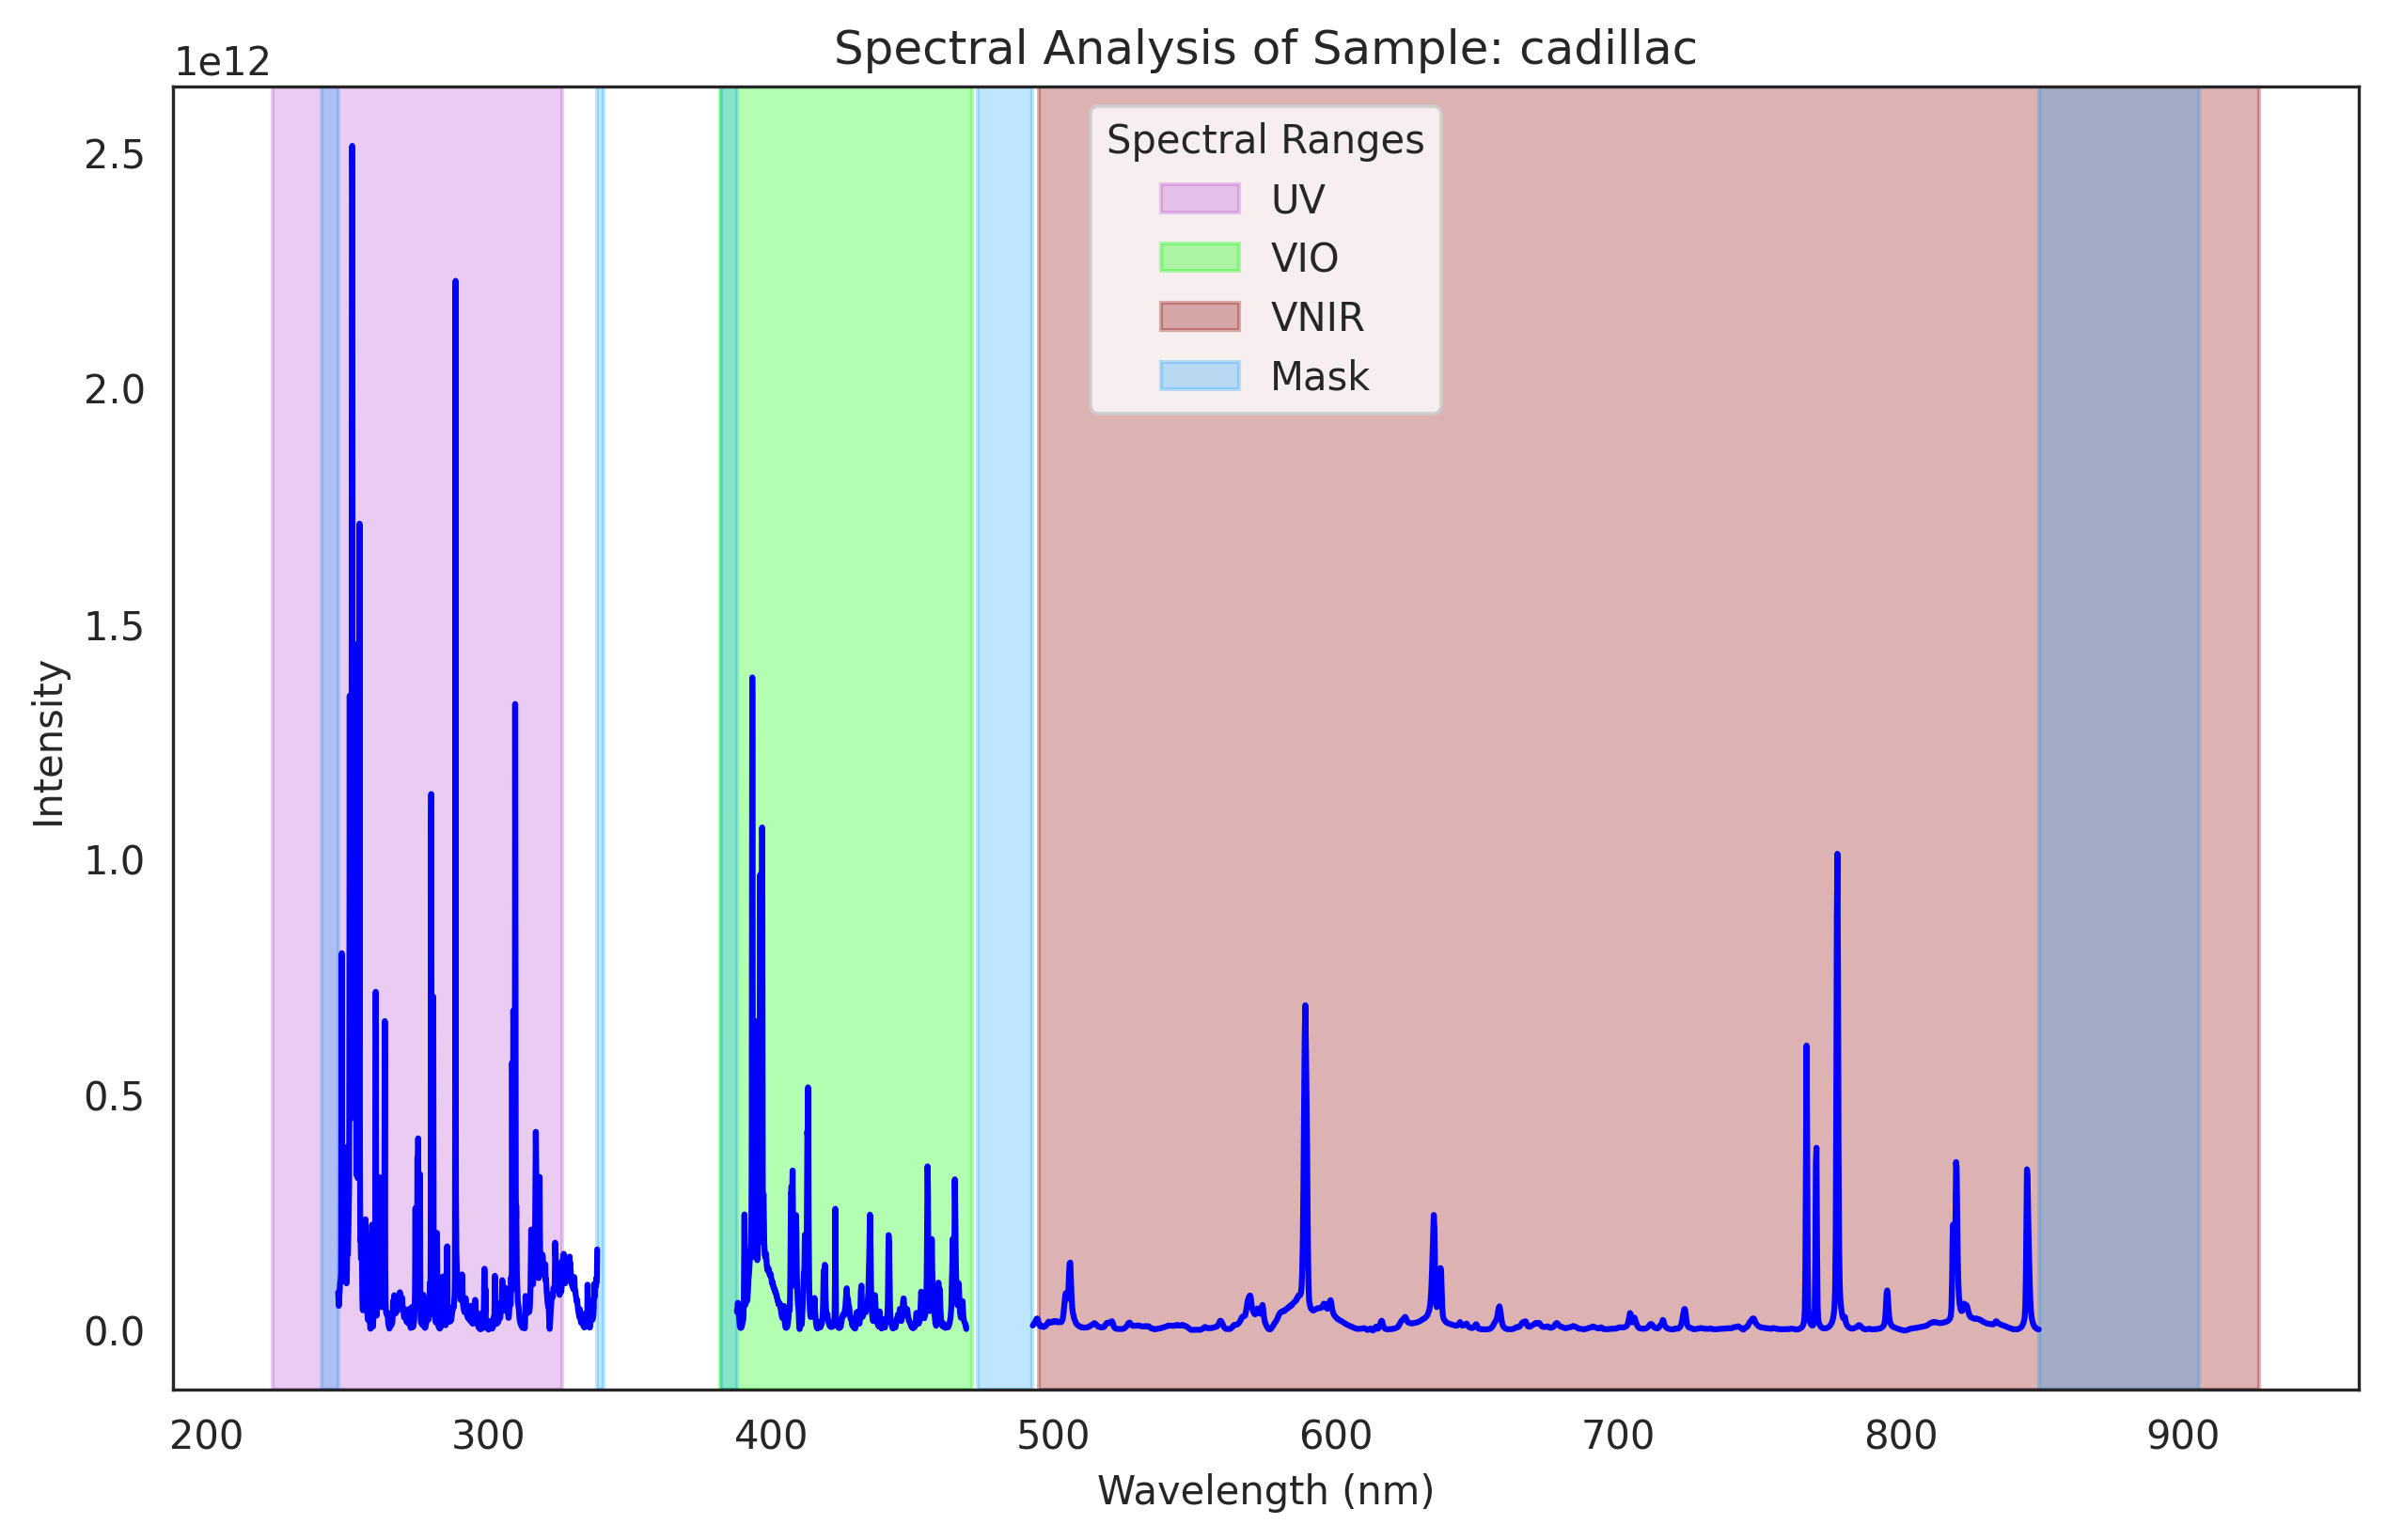
\includegraphics[width=0.5\textwidth]{images/masked_regions.png}
	\caption{Spectral plot of the CCS data for the \texttt{cadillac} sample. The blue regions represent the noisy edges of the spectral regions.}
	\label{fig:masked_regions}
\end{figure}

In addition to these datasets, there is also a \\ \texttt{ccam\_calibration\_compositions.csv} file that contains ground truth data for each major oxide in each sample.
There are a total of eight major oxides: \ce{SiO2}, \ce{TiO2}, \ce{Al2O3}, \ce{FeOT}, \ce{MnO}, \ce{MgO}, \ce{CaO}, \ce{Na2O}, and \ce{K2O}.
For each of these oxides, the data specifies their respective concentrations in each sample, expressed as a weight percentage (wt. \%) of the total composition.